\chapter{Implementation}
\label{chap:implementation}

In this chapter, we will delve into the implementation details of the presented visualizations applied in our experimental application called MeshDiff. We will also describe the overall architecture of MeshDiff.

%%-----------------------------------------------------------------------------------------
%% SECTION
%%-----------------------------------------------------------------------------------------
\section{Visualization Algorithm}
\label{sec:implementation-algorithm}

All presented visualizations share a common workflow (algorithm) in MeshDiff. In this section, we will discuss all parts of the workflow, namely:

\begin{itemize}
\item Difference metric computation
\item Vector clustering
\item Cluster visualization
\end{itemize}

First, however, we will describe the internal representation of triangle meshes in MeshDiff and the framework that the visualization algorithm fits into.

%%-----------------------------------------------------------------------------------------
\subsection{Triangle Mesh Representation}
\label{subsec:implementation-algorithm-mesh_repre}

We are using an implementation of triangle mesh boundary representation with a corner table which was presented in \citet{Corner03}. The implementation was written by Josef Pelikán. For brevity, we will refer to this representation as a {\it scene}.

\begin{figure}[h]
\centering
\def\svgwidth{0.5\textwidth}
\input{./illustrations/corner_table.pdf_tex}
\caption[Corner Table Illustration]{An illustration of the corner table. The black corner has direct access to all red elements - its vertex and certain surrounding corners}
\label{fig:illustration-corner_table}
\end{figure}

In this representation, we do not primarily store the vertices of the triangle mesh but the corners of the triangles. The corner table then allows us to obtain certain surrounding corners of a given corner and associated vertices in constant time. This makes traversing an arbitrary triangle mesh very simple and fast.

We have added several methods to this implementation in order for us to be able to quickly obtain the list of neighbors of a given vertex and compute the geometrical area of clusters.

%%-----------------------------------------------------------------------------------------
\subsection{Algorithm Framework}
\label{subsec:implementation-algorithm-framework}

The core class of MeshDiff which encapsulates the visualization algorithm is called \verb+DiffAlgo+. \verb+DiffAlgo+ is initialized by the {\it rendered scene} and the {\it reference scene} and therefore only operates on these two specific {\it scenes} throughout its whole lifetime.

The main public method of \verb+DiffAlgo+ is \verb+CreateVisualization()+. It is mainly responsible for metric computation and vector\footnotemark clustering. All this computed data is stored inside \verb+DiffAlgo+ instances. When the clustering is ready, a visualization is created and outputted from \verb+CreateVisualization()+ using a visualizer object.

\footnotetext{As mentioned in \ref{sec:analysis-input}, all our difference metrics can be represented by a vector.}

The fact that all intermediate results are stored inside a \verb+DiffAlgo+ instance means that when \verb+CreateVisualization()+ is called again, data which is difficult to compute, especially the vector clustering, can be reused if possible.

The C\#-styled\footnotemark pseudocode below describes the visualization workflow which will be further discussed in the following sections.

\footnotetext{The \verb+ref+ keyword used with method arguments is meant to emphasize that a value is returned via these arguments.}

\begin{algorithm}[H]
\caption{CreateVisualization()}
\label{algo:create_vis}
\begin{algorithmic}[1]

\Require metricType, clusteringParams, visParams, visualizer, ref outputScene1, ref outputScene2 \Comment other variables are contained in the DiffAlgo object
\Statex
\Statex \Comment Difference metric computation
\If{required metric values not available}
	\State arrows = GetArrows(renderedScene, refScene, metricType);
    \State clusteringObject = ClusteringFactory(arrows, sceneP);
    \State currentMetricType = metricType;
\EndIf
\Statex \Comment Vector clustering
\State clusters = clusteringObject.GetClusters(clusteringParams);
\Statex \Comment Cluster visualization
\State visualizer.BakeVis(clusters, visParams, ref outputScene1);
\State visualizer.BakeVisInv(clusters, visParams, ref outputScene2);
\Statex
\Return
\end{algorithmic}
\end{algorithm}

%%-----------------------------------------------------------------------------------------
\subsection{Difference Metric Computation}
\label{subsec:implementation-algorithm-metrics}

In order to compute a difference metric, this part of the workflow requires the type of the metric it should compute and also both {\it scenes}. The former is passed in as an argument of \verb+CreateVisualization()+ and the latter are stored inside \verb+DiffAlgo+.

As mentioned earlier, we have included two difference metrics in MeshDiff, both of which can be represented by a 3D vector:

\begin{itemize}
\item Corresponding vertex distance
\item Corresponding vertex distance projected into surface normal
\end{itemize}

We have created a common representation for both of these metrics called \verb+Arrow+ which encapsulates a 3D vector, its origin and other useful data and acts as input to the clustering algorithm.

Here are the most important fields of \verb+Arrow+:

\begin{itemize}
\item \verb+Origin+ - the position of the vector metric, initially coinciding with a {\it scene} vertex (this can change during the clustering process)
\item \verb+Direction+ - a 3D vector representing the metric itself
\item \verb+Orientation+ - tells whether the arrow points {\it inwards} or {\it outwards}
\item \verb+VertexHandle+ - if \verb+Origin+ coincides with a {\it scene} vertex, this is its index in the {\it scene} representation, otherwise it is -1
\end{itemize}

If the required metric type is equal to the current metric type stored in \verb+DiffAlgo+, old data is reused and this step is skipped, otherwise all corresponding vertices of both {\it scenes} are enumerated and for each pair, the configured metric is computed on the {\it rendered scene} and relative to the {\it reference scene}. For example, in the case of corresponding vertex distance, consider a {\it rendered scene} \(S_p\), a {\it reference scene} \(S_r\), vertices (vectors) \(\overrightarrow{v} \in S_p, \overrightarrow{w} \in S_r\) and a difference metric vector \(\overrightarrow{m}\). Then \(\overrightarrow{m_{vw}} = w - v\). Therefore, \(m_{vw}\) behaves as shown in Fig. \ref{fig:illustration-problem_input}.

\subsubsection{Output}

A list of \verb+Arrow+ instances indexed by the handles of the corresponding vertices in the {\it rendered scene}.

%%-----------------------------------------------------------------------------------------
\subsection{Vector Clustering}
\label{subsec:implementation-algorithm-clustering}

The clustering step requires the list of \verb+Arrow+ instances from the previous step, the clustering parameters (see attachment \ref{attch:parameter_desc-clustering_parameters}) and, most importantly, the clustering type. The parameters are passed in as arguments of \verb+CreateVisualization()+. We will now talk about the clustering type.

As mentioned in \ref{subsec:analysis-field_clustering-our_method}, our clustering has two types. For the sake of implementation consistency, we also introduce a third type, the ``empty'' clustering, which does not reduce the number of vectors in any way and can be used when no clustering is needed. Each clustering type has an associated class, all of which share a common interface.

Overall, there are three clustering types in MeshDiff:

\begin{itemize}
\item None
\item {\it Simple}
\item {\it Signed}
\end{itemize}

The clustering type used in \verb+DiffAlgo+ is determined by a factory method passed to its constructor. A \verb+DiffAlgo+ instance can therefore create and use the clustering object without knowing its type and at the same time it is limited to using only one clustering type. Thanks to this, computed clusterings of multiple types can be saved simultaneously (in different \verb+DiffAlgo+ instances) and reused if needed. It is important to note that this reuse happens every time the user chooses to view a new visualization which differs from the previous one only in the number of clusters to be generated, thanks to the dendrogram (see Fig. \ref{fig:illustration-telea_hierarchical_clustering}) which contains all clusterings of 1 to \(n\) clusters where \(n\) is the number of original arrows. When a reuse is impossible, a new clustering object is created using the factory method. Another reason why this encapsulation approach was chosen is that dendrograms should be stored in the clustering objects and not in the \verb+DiffAlgo+ instances in order for the implementation details to stay hidden from \verb+DiffAlgo+.

We will now introduce a new class called \verb+Cluster+ which \verb+Arrow+ instances are converted to in the clustering process and whose instances form nodes of the dendrogram. \verb+Cluster+ instances are able to merge with other \verb+Cluster+ instances and compute the clustering error given another \verb+Cluster+ instance. They also contain all the information needed for the visualization to be created. Here are the most important fields of \verb+Cluster+:

\begin{itemize}
\item \verb+Neighbors+ - a set of \verb+Cluster+ instances adjacent to the cluster
\item \verb+Level+ - marks the step of the clustering algorithm in which this cluster was created (low number also means low clustering error in general), it is illustrated in Fig. \ref{fig:illustration-telea_hierarchical_clustering}
\item \verb+RepresentativeArrow+ - an \verb+Arrow+ instance representing the metric value for this cluster
\item \verb+Size+ - the geometrical area of the cluster. We have chosen this to be the sum of the areas of the underlying mesh triangles which belong to the cluster
\item \verb+LeftChild+ and \verb+RightChild+ - \verb+Cluster+ instances out of which this cluster was created
\item \verb+PrimaryArrows+ - a list of all the original unclustered \verb+Arrow+ instances which are tied directly to the underlying {\it scene} and which belong to this cluster
\end{itemize}

\verb+Cluster+ instances can be sorted and the sorting field is \verb+Level+.

If the new \verb+Arrow+ instances are the same as the current ones \verb+DiffAlgo+ contains, the old clustering object is reused. Otherwise, the factory method is used to initialize a new clustering object with the new \verb+Arrow+ instances. After that, clustering parameters including the required cluster count are passed to the clustering object. The clustering object checks if it already has a clustering corresponding to the given parameters and if it does, it simply extracts the required number of clusters from the available dendrogram and returns them. This is how the extraction works when the dendrogram is a tree\footnote{Corresponds to {\it simple clustering.}}:

\begin{algorithm}[H]
\caption{Cluster Extraction from a Tree}
\label{algo:cluster_extract-tree}
\begin{algorithmic}[1]

\Require MaxHeap chosenClusters, requiredClusterCount
\Statex
\State chosenClusters.Clear();
\State chosenClusters.Insert(dendrogram root);
\State i = 0;
\While{i < requiredClusterCount}
	\State highestCluster = chosenClusters.ExtractMax();
    \State chosenClusters.Insert(highestCluster.LeftChild);
    \State chosenClusters.Insert(highestClusters.RightChild);
    \State i++;
\EndWhile
\Statex
\Return chosenClusters as list
\end{algorithmic}
\end{algorithm}

Here is the extraction algorithms for forest dendrograms\footnote{Corresponds to {\it signed clustering.}}:

\begin{algorithm}[H]
\caption{Cluster Extraction from a Forest}
\label{algo:cluster_extract-forest}
\begin{algorithmic}[1]

\Require MaxHeap chosenClusters, requiredClusterCount
\Statex
\State chosenClusters.Clear();
\State chosenClusters.Insert(all dendrogram roots);
\State i = 0;
\While{i < requiredClusterCount}
	\State highestCluster = chosenClusters.ExtractMax();
	\If{highestCluster.Level == 0}
		\State chosenClusters.Insert(highestCluster);
		\State \textbf{break};
	\EndIf
    \State chosenClusters.Insert(highestCluster.LeftChild);
    \State chosenClusters.Insert(highestClusters.RightChild);
    \State i++;
\EndWhile
\State list = chosenClusters.ExtractMaxNTimes(requiredClusterCount);
\Statex
\Return list
\end{algorithmic}
\end{algorithm}

The condition on line 6 of algorithm \ref{algo:cluster_extract-forest} is fulfilled for example when five clusters are requested from the forest in Fig. \ref{fig:illustration-forest_dendrogram}. In this case, \verb+highestCluster+ is a root without any children. At the same time, however, all of these roots have already been added to \verb+chosenClusters+ on line 2. We therefore insert the \verb+highestCluster+ back and break the loop because there are no more clusters to discover. We will remove the redundant clusters in the next step.

Line 12 of algorithm \ref{algo:cluster_extract-forest} ensures that clusters which were chosen only because they are roots (line 2) and not because their level is high enough are excluded from the selection. This is necessary to return the cluster count requested but at the same time it introduces the limitation we discussed in section \ref{subsec:analysis-field_clustering-our_method} which is that for certain cluster counts, the returned clusters do not cover the whole {\it scene}.

If the desired clustering is not available (i.e. the corresponding dendrogram is not built), the clustering object performs the clustering algorithm. Here is the outline of it (largely similar to \citet{Telea99}):

\begin{algorithm}[H]
\caption{Clustering}
\label{algo:clustering}
\begin{algorithmic}[1]

\Require arrows, MinHeap clusteringCandidates \Comment clusteringCandidates are ordered by clustering error
\Statex
\For{each arrow\textsubscript{i} \textbf{in} arrows}
	\State initialCluster = makeCluster(arrow\textsubscript{i});
    \State set level of intialCluster to 0;
    \State add initialCluster to initialClusters;
\EndFor
\Statex
\For{each cluster\textsubscript{i} in initialClusters}
	\For{each cluster\textsubscript{j} neighbour of cluster\textsubscript{i}}
    	\State e = clusteringError(cluster\textsubscript{i}, cluster\textsubscript{j});
        \State insert (cluster\textsubscript{i}, cluster\textsubscript{j}) into clusteringCandidates
        \State mark cluster\textsubscript{i} and cluster\textsubscript{j} as NOT\_CLUSTERED;
    \EndFor
\EndFor
\Statex
\State level = 0;
\While{clusteringCandidates.Count > 0}
	\State (cluster\textsubscript{i}, cluster\textsubscript{j}) = clusteringCandidates.ExtractMin();
    \If{cluster\textsubscript{i} and cluster\textsubscript{j} are both NOT\_CLUSTERED}
    	\State newCluster = mergeClusters(cluster\textsubscript{i}, cluster\textsubscript{j});
        \State set level of newCluster to level++;
		\State mark newCluster as NOT\_CLUSTERED;
        \State mark cluster\textsubscript{i} and cluster\textsubscript{j} as CLUSTERED;
        \For{each cluster neighbour of newCluster}
        	\State e = clusteringError(cluster, newCluster);
            \State insert (cluster, newCluster) into clusteringCandidates
        \EndFor
    \EndIf
\EndWhile
\Statex
\Return c as root of tree
\end{algorithmic}
\end{algorithm}

\verb+mergeClusters()+ and \verb+clusteringError+ are implemented in accordance with section \ref{subsec:analysis-field_clustering-our_method}. We will now mention the most important implementation details of \verb+mergeClusters()+.

First of all, when a new cluster is created, it needs to be placed in the clustering space by modifying all neighboring clusters of its two children to be the neighbors of the new cluster instead, except for the children themselves. Also, the neighboring relation has to be made symmetrical by updating the neighbor lists of the surrounding clusters. The orientation of the new representative arrow is either inherited ({\it signed clustering}) or estimated based on the dominant orientation among the \verb+PrimaryArrows+ of the new cluster. New mesh resolution is obtained by averaging the resolutions of the two original clusters. Lastly, the size of the new cluster is computed directly when the cluster is sufficiently small, otherwise it is determined by the sum of the sizes of the original clusters.

\subsubsection{Output}

A list of \verb+Cluster+ instances is returned, even in the case of ``empty'' clustering where the only operation is the conversion of \verb+Arrow+ instances into \verb+Cluster+ instances.

%%-----------------------------------------------------------------------------------------
\subsection{Cluster Visualization}
\label{subsec:implementation-algorithm-visualization}

When the visualization itself is to be generated from the list of \verb+Cluster+ instances, visualization parameters (see attachment \ref{attch:parameter_desc-visualization_parameters}), a visualizer object and two output {\it scenes} are required. \verb+CreateVisualization()+ receives all of these as arguments. We will now talk about visualizer objects.

In section \ref{sec:analysis-visualizations}, we have proposed several types of visualizations. Each of them has an associated visualizer object which generates it based on \verb+Cluster+ instances supplied to it. It is useful to compare these objects with clustering objects described in section \ref{subsec:implementation-algorithm-clustering} because both are utilized differently in \verb+DiffAlgo+.

Clustering objects are designed to store dendrograms for potential later reuse because their computation is time-consuming and a reuse is likely. Visualizer objects, on the other hand, do not store any state or intermediate results because visualizations are fast to compute and reuses are not very helpful because outputting a visualization requires similar time as creating it. They can therefore be passed to \verb+CreateVisualization()+ from the outside and used only to directly output visualizations.

All visualizer objects have two public methods, one is intended for visualizations for the {\it rendered scene} and the other is intended for visualizations for the {\it reference scene}. The latter is obtained by inverting the former. See Fig. \ref{fig:illustration-problem_input} for an illustration of the situation. Creating visualizations for both of the compared scenes allows for both of them to be displayed next to each other which enhances the effect of the visualizations. See Fig.\ref{fig:meshdiff-inverted_vis}.

\begin{figure}[h]
\centering
	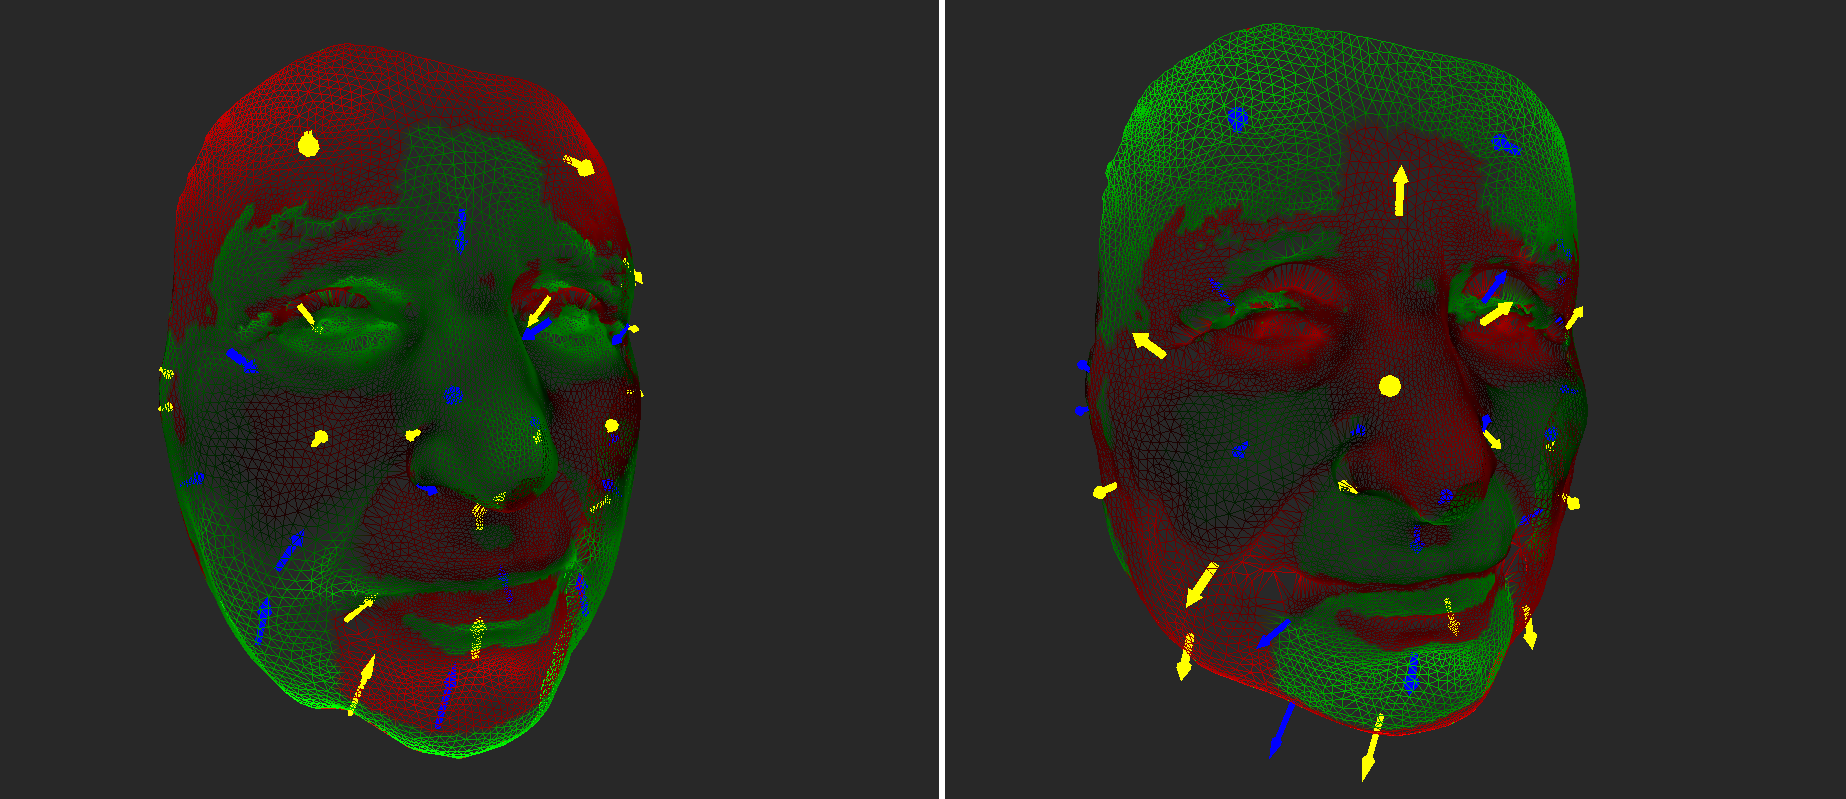
\includegraphics[width=\textwidth]{./img/mesh_diff-inverted_vis.png}
    \caption[MeshDiff - Two mutually inverted visualizations]{MeshDiff - Two mutually inverted visualizations displayed next to each other}
    \label{fig:meshdiff-inverted_vis}
\end{figure}

We will now focus on two main types of visualizers - arrow visualizers and color visualizers - and the way they bake the visualization into the output {\it scenes} mentioned in algorithm \ref{algo:create_vis}.

\subsubsection{Arrow Visualizers}

Arrow visualizer objects only have one field which is initialized in the constructor. This field holds a basic {\it scene} representing a 3D arrow. The triangle mesh of this arrow was created manually in order to have the least amount of vertices and triangles possible to reduce the overall amount of data. It has 17 vertices and 16 triangles. The tip of the arrow is an eight-sided pyramid which was found to have much better appearance than the basic four-sided pyramid and this justified the slightly larger vertex count.

\begin{figure}[h]
\centering
	\begin{subfigure}{0.3\textwidth}
	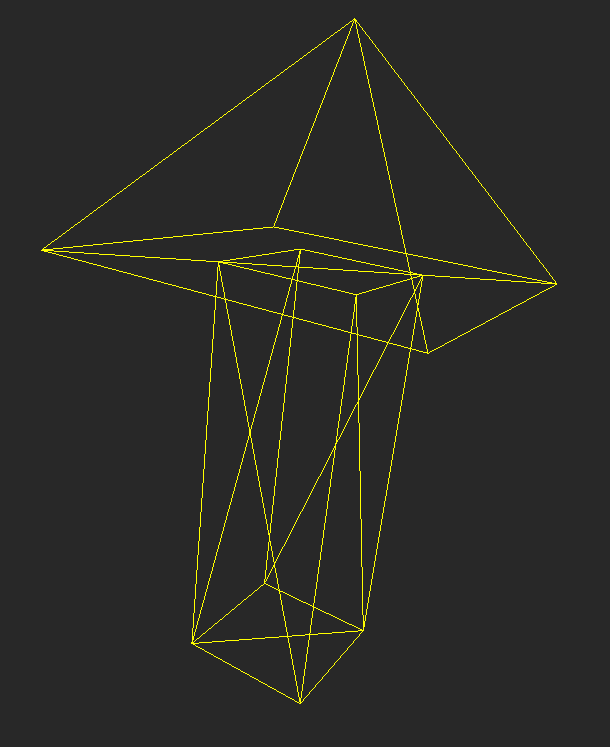
\includegraphics[width=\textwidth]{./img/4sided_arrow.PNG}
    \caption{Four-sided tip version (not used)}
    \label{fig:meshdiff-4sided_arrow}
	\end{subfigure}
    \qquad
    \begin{subfigure}{0.3\textwidth}
	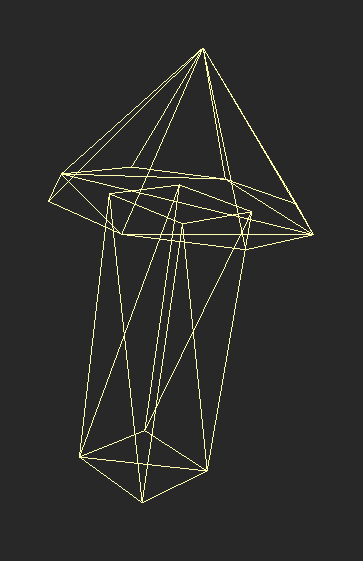
\includegraphics[width=\textwidth]{./img/8sided_arrow.PNG}
    \caption{Eight-sided tip version (used)}
    \label{fig:meshdiff-8sided_arrow}
	\end{subfigure}
\caption[Wireframe models used for arrow visualizations]{Wireframe models used for arrow visualizations}
\end{figure}

The visualizer receives a list of clusters as input, loops through those which passed through thresholding and makes a scaled copy of the basic arrow in each iteration. The scale of the copy is based on the representative vector of the cluster as described in section \ref{subsec:analysis-visualizations-arrows} and on the visualization parameters supplied. Colors are assigned to the arrow {\it scenes} depending on whether the representative vector points {\it inwards} or {\it outwards} (see attachment \ref{attch:parameter_desc-visualization_parameters}). All created arrow {\it scenes} are then copied into the output {\it scene} supplied.

The inverted visualization is obtained by multiplying the representative vector by -1 and assigning the arrow {\it scene} colors based on this version of the vector.

\subsubsection{Color Visualizers}

For each color visualization type mentioned in section \ref{sec:analysis-visualizations} there is a separate visualizer class. These classes determine how color is assigned to vertices. In general, each visualizer loops though all \verb+Cluster+ instances supplied and for each of them it generates a color based on the metric value for that cluster. Clusters which passed through thresholding receive a color based on the length of the representative vector and its orientation (see attachment \ref{attch:parameter_desc-visualization_parameters}). Once a color is created, it is inserted into a list at precisely those indices which belong to the \verb+PrimaryArrows+ (see section \ref{subsec:implementation-algorithm-clustering}) of the associated cluster. It is important to respect this indexing in order to make the mapping of the colors to the {\it scene} vertices easier. The colors are then applied to the vertices of the output {\it scene} supplied\footnotemark.

The inverted visualization is also obtained by multiplying the representative vector by -1 and generating the colors based on this version of the vector.

\footnotetext{It is worth mentioning that when the clusters supplied to this visualizer correspond to the original vectors (i.e. no clustering was performed), a per-vertex visualization is generated similar to those in MeshLab or Morphome3cs (see the introduction).}

\subsubsection{Output}

The generated visualization is baked into the first supplied output {\it scene} and an inverted visualization is baked into the second supplied {\it scene}.
%%-----------------------------------------------------------------------------------------
%% SECTION
%%-----------------------------------------------------------------------------------------
\section{MeshDiff Architecture}
\label{sec:implementation-architecture}

Similarly to MeshLab or Morphome3cs, in MeshDiff, the core functionality is the ability to load and store triangle meshes and to view them interactively using the mouse cursor. Because this functionality is present in almost all programs which work with triangle meshes and at the same time it is non-trivial, we reused available code which provides it, more specifically we built MeshDiff on top of a mesh viewer application written by Josef Pelikán.

In this chapter, we will mention the platform MeshDiff is built on and intended for, then we will talk about the features we added to the reused mesh viewer and the changes we made to the user interface to support of visualization rendering purposes. At the end, we will reveal how the visualization workflow is incorporated into MeshDiff.

%%-----------------------------------------------------------------------------------------
\subsection{Platform}
\label{subsec:implementation-architecture-platform}

The reused code by Josef Pelikán is a C\# application with a WinForms user interface which uses the OpenTK library, encapsulating the OpenGL API, to render graphics. The only targeted operating system is Windows which is sufficient for our experimental purposes.

In order to clearly mark which parts of MeshDiff are authored by us and which are reused, we have stated the origin of the code in each source file and in this thesis, we will use the terms {\it resued code} and {\it original code} to differentiate between the two.

%%-----------------------------------------------------------------------------------------
\subsection{Triangle Mesh Viewing}
\label{subsec:implementation-architecture-mesh_viewing}

The {\it reused code} of MeshDiff supports two standard triangle mesh formats, \verb+.obj+ and \verb+.ply+. It is able to load and store files in these formats and also convert between them and the internal {\it scene representation} (see section \ref{subsec:implementation-algorithm-mesh_repre}) of a triangle mesh. The {\it scene} can be prepared for rendering by storing its data in the vertex buffer object in the GPU. This is accomplished by calling one of the {\it scene's} own methods. In each frame, a rendering method is called which comprises OpenTK calls tied to a view panel showing the triangle mesh. The view panel is a custom OpenTK control placed directly in the main form of the application. This process can be configured by a set of toggles which can change the viewing mode to wireframe, enable shading, etc.

Interactivity is handled by a class called \verb+Trackball+ which intercepts mouse events from the view panel and modifies the model matrix used in the rendering process.

We have added several modifications to this basic setup to support the rendering of visualizations of the difference between two triangle meshes. Here are the most significant ones:

\begin{itemize}
\item We have added a second viewing panel for the inverted visualization on the {\it reference mesh} (see section \ref{subsec:implementation-algorithm-visualization}). This required duplicating the buffer objects, \verb+Trackball+ instances and also fields which stored the loaded {\it scenes}.
\item Based on that we have added the option to either control both views separately, or to control both of them at the same time. This is done by first modifying the \verb+Trackball+ instance according to the mouse event associated with the view panel in was intended for and then copying the resulting rotation matrix from that instance to the second instance. Because the coordinates in the mouse events are tied to their view panels, simply routing the events to the second view panel would only work if both panels had the same dimensions. This solution is more general and bypasses coordinate recalculation.
\item When visualizations are to be created, the visualizer objects (see section \ref{subsec:implementation-algorithm-visualization}) are supplied with copies of the raw {\it scenes} to bake the visualizations to. These visualization {\it scenes} are then stored alongside the raw scene. This allows users to quickly switch between viewing visualizations and raw {\it scenes}. When a new visualization is requested, another pair of copies is be made out of the raw {\it scenes} and when the visualization is baked, it replaced the old visualization pair.
\item For the case when arrows are part of a visualization, we have added the option to toggle wireframe view independently for them and the underlying {\it scene}. The arrows therefore need to be stored in a separate {\it scene} and the option to render two {\it scenes} at once was added to the rendering methods. In the visualization process, this is achieved by baking the color visualization into the underlying {\it scene} and the arrow visualization into an empty {\it scene} (see section \ref{subsec:implementation-algorithm-visualization}).
\end{itemize}

\begin{figure}[h]
	\centering
	\def\svgwidth{\textwidth}
	\input{./illustrations/scenes_explained.pdf_tex}
	\caption[Scenes Explained]{An illustration of the two view panels of MeshDiff and various scenes which can be displayed in them.}
	\label{fig:illustration-scenes_explained}
\end{figure}

To summarize, next to the pair of raw {\it scenes} we also store four additional {\it scenes}: one pair for the raw {\it scenes} with color visualizations and one pair only for arrows. See Fig. \ref{fig:illustration-scenes_explained} for an illustration of this.

%%-----------------------------------------------------------------------------------------
\subsection{User Interface}
\label{subsec:implementation-architecture-user_interface}

We have extended the {\it reused} user interface by adding functionality which allows the user to configure the visualization before it is generated. For the complete description of the configuration options, see attachment \ref{attch:parameter_description}. The user can also save this configuration to a file or load it from a file. See attachment \ref{attch:parameter_load_store} for more details on this.

We have decided to duplicate clustering parameters and have a separate set for clustering in color visualizations and arrow visualizations. This makes MeshDiff more flexible because if there was only one set, it would not be possible to visualize using unclustered color and clustered arrows at the same time.

The most important clustering and visualization parameters can be modified directly from the main form where both triangle meshes can be viewed interactively as well. Metric type and all other parameters have their separate dialog windows.

There are four places in the code where this configuration is held. The \verb+Trackball+ class remembers the model matrix and zoom value for each of the displayed triangle meshes. Currently chosen difference metric type is stored in a single variable. Clustering parameters have their own dedicated class and so do the visualization parameters which control the appearance of the visualizations.

Apart from being able to pass the parameters to the \verb+DiffAlgo+ class in a compact way, this approach also has the advantage that each class encapsulating a certain group of parameters is also able to write them to a file and it is also able to initialize itself from a file\footnotemark.

\footnotetext{Metric type is stored in a variable but there is a dedicated class called \verb+Metric+ in the program which handles metric computation and on top of that is also able to handle the input/output operations.}

Each of the parameter classes implement individual parameters as properties and handle value checks. Exceptions thrown by these checks are not being caught, however, because the user interface is designed in such a way that invalid values cannot be assigned. Invalid assignments from code are then correctly detected and an exception is thrown in such cases.
%%-----------------------------------------------------------------------------------------
\subsection{Visualization Infrastructure}
\label{subsec:implementation-architecture-infrastructure}

The visualization is purely handled by our {\it original code}. Once the user has finished their configuration and started the visualization generation, an asynchronous job is initialized to handle this process in a user-friendly way.

The behavior of the job is fully determined by a configuration package class called \verb+JobParameters+. Here is the full list of its fields:

\begin{itemize}
\item \verb+DiffForColors+ - A \verb+DiffAlgo+ instance which handles clustering for color visualization
\item \verb+DiffForArrows+ - A \verb+DiffAlgo+ instance which handles clustering for arrow visualization
\item \verb+Metric+ - Metric type
\item \verb+ClusteringParametersArrows+
\item \verb+ClusteringParametersColors+
\item \verb+VisualizationParameters+
\item \verb+VisualizerColor+ - Color visualizer object
\item \verb+VisualizerArrow+ - Arrow visualizer object
\item \verb+Scene1Color+ - The {\it rendered scene} for color visualization baking
\item \verb+Scene2Color+ - The {\it reference scene} for inverted color visualization baking
\item \verb+Scene1Arrows+ - The {\it rendered scene} (or an empty {\it scene}) for arrow visualization baking
\item \verb+Scene2Arrows+ - The {\it reference scene} (or an empty {\it scene}) for inverted arrow visualization baking
\end{itemize}

The are two \verb+DiffAlgo+ instances to support different clustering for arrow visualization and color visualization as described in section \ref{subsec:implementation-architecture-user_interface}.

Once a job is initialized with this package, its \verb+Run()+ method can be assigned to a thread. A job operates directly with the \verb+DiffAlgo+ class, initializes it and calls its methods according to the configuration package. The thread is started together with a dialog window which shows progress and enables the user to cancel the process. Once the visualization process finishes, the program checks whether it has finished successfully or not and assigns based on that either renders the computed visualization {\it scenes} or reports an error and renders the previously shown {\it scenes}.

Checking for visualization cancellation is done mainly during the clustering loop because it is the most time-consuming part of the program. It is also done after the visualization is generated because otherwise the process would finish even when the user has requested a cancellation. When a process is canceled, all the intermediate data related to that process is deleted and the previously shown {\it scenes} are rendered.